\documentclass{article}
\usepackage[margin=2cm]{geometry}
\usepackage{tikz}
\begin{document}
\section*{Cyberdisc rotating-collider admission}
Created-at: 2026-10-05 03:21 CEST. ETA: 25 minutes (focused regression, small
owner fix, targeted checks and report). No benchmark or simulation campaign.

\paragraph{Owner and scope} Transformation/Formats owns the generated-world
actor admission. Geometry owns collision primitives and forward kinematics;
Robotics owns the unchanged actor. Reuse these owners. A collider offset may
point inward at zero wheel angle and outward after half a revolution. Replace
the zero-pose centre norm with the conservative triangle bound: distance from
chassis to link origin plus offset norm plus existing shape bound.

\paragraph{Acceptance} First reproduce old admission of the shifted-wheel
fixture, while existing FK shows its half-turn envelope exceeds the cell
clearance. The fixed admission rejects it. The unchanged zero-offset actor
retains the exact previous envelope and the existing small-world export passes.
This bounds collider rotation about its link; no general articulated sweep or
dynamic route-following guarantee is claimed.

\paragraph{Files} Existing
\texttt{hymeko\_formats/examples/adversarial\_grid/physical.rs}; this plan bundle;
\texttt{reports/2026-10-05-rotating-collider-envelope.md} and its raw logs.
CORE.YAML items touched: []. No public signatures, schema, dependency, actor,
controller or physics changes. Existing 64-obstacle, 32-waypoint, 2m-cell caps
and 0.16m arrival tolerance remain unchanged.

\paragraph{Checks and budget} Pure FK regression on local Rust, exact ignored
sibling actor integration tests, ordinary grid correctness tests and Clippy.
No rollout, inference, performance measurement or generated-world ranking.
At most two build jobs; each check bounded externally to 180s where practical.
No package installation, worktree, commit or push. Worst-case accepted profile
remains 16x16 cells, 64 obstacles and 32 waypoints.

\paragraph{Risks} Conservative triangle inequality may refuse an offset actor
that would fit; this is explicit admission conservatism. Bounds rely on the
existing shape owner and reusable Cyberdisc layout, not arbitrary articulated
chains. Existing zero offsets must preserve the old result exactly.
Rollback consists of reverting this isolated source delta after review; no
automatic destructive operation is performed.

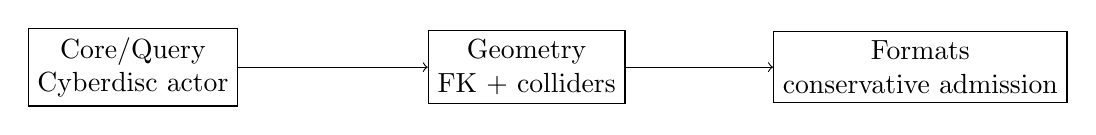
\begin{tikzpicture}[every node/.style={draw,align=center}]
\node (ir) at (0,0) {Core/Query\\Cyberdisc actor};
\node (fk) at (5,0) {Geometry\\FK + colliders};
\node (admit) at (10,0) {Formats\\conservative admission};
\draw[->] (ir) -- (fk); \draw[->] (fk) -- (admit);
\end{tikzpicture}

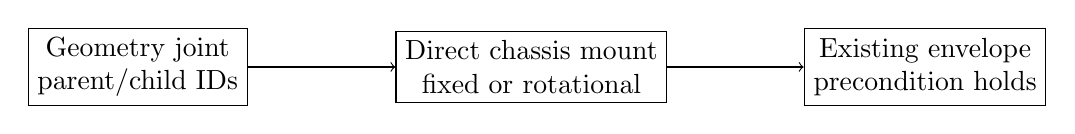
\begin{tikzpicture}[every node/.style={draw,align=center}]
\node (relation) at (0,0) {Geometry joint\\parent/child IDs};
\node (profile) at (5,0) {Direct chassis mount\\fixed or rotational};
\node (bound) at (10,0) {Existing envelope\\precondition holds};
\draw[->] (relation) -- (profile); \draw[->] (profile) -- (bound);
\end{tikzpicture}

\section*{Continuation: collider mount assumptions}
Created-at: 2026-10-05 21:13 CEST. ETA: 25 minutes, based on two pure FK
counterexamples, a private admission check, regression tests, and reporting.

\paragraph{Hypothesis} The offset norm bound assumes that each collider link's
origin remains at fixed distance from the chassis. The admitted source currently
permits nesting a wheel under another driven wheel or making its mount prismatic.
At zero configuration these may fit, then leave the corridor under joint motion.

\paragraph{Discriminating check} Compile controlled changes to the existing actor;
use owner FK and support queries at zero and one nonzero joint value. Preserve
before-fix false admission in logs. If reproduced, require every non-chassis
collision-bearing link to have a direct fixed/rotational mount on the chassis,
using canonical declaration IDs and projected JointType. This checks the actual
existing Cyberdisc profile; no general robot importer or articulated sweep is added.

\paragraph{Acceptance and boundaries} Both invalid mounts fail before output
creation. Existing actor/export, shifted-offset regression, and grid tests pass.
Clippy, format, diff and provider duplication checks apply. CORE.YAML: []. Same
source file, this existing plan/report, and a new mount-admission evidence subfolder.
No dependency, schema, controller or engine changes. No Mission Control access.
No simulation is needed to establish static geometric counterexamples; any later
simulation remains Amaterasu-only. Two build jobs, 180-second command ceiling,
no benchmark/profiling, no commit/push/merge/worktree. Preserve prior dirty edits.

\paragraph{Risk} This intentionally refuses nested and translating collider
mounts, including configurations that could fit. Fixed/rotational direct mounts
are sufficient for the current envelope; arbitrary actors remain outside scope.
Rollback removes only this continuation's reviewed delta, preserving the earlier fix.
\end{document}
